%!TEX program = xelatex

\documentclass[a4paper, openany, oneside]{memoir}
\usepackage[no-math]{fontspec}
\usepackage{pgfplots}
\pgfplotsset{compat=newest}
\usepackage{commath}
\usepackage{mathtools}
\usepackage{amssymb}
\usepackage{amsthm}
\usepackage{booktabs}
\usepackage{mathtools}
\usepackage{xcolor}
\usepackage[separate-uncertainty=true, per-mode=symbol]{siunitx}
\usepackage[noabbrev, capitalize]{cleveref}
\usepackage{listings}
\usepackage[american inductor, european resistor]{circuitikz}
\usepackage{amsmath}
\usepackage{amsfonts}
\usepackage{ifxetex}
\usepackage[dutch,english]{babel}
\usepackage[backend=bibtexu,texencoding=utf8,bibencoding=utf8,style=ieee,sortlocale=en_GB,language=auto]{biblatex}
\usepackage[strict,autostyle]{csquotes}
\usepackage{parskip}
\usepackage{import}
\usepackage{standalone}
\usepackage{hyperref}
%\usepackage[toc,title,titletoc]{appendix}

\ifxetex{} % Fonts laden in het geval dat je met Xetex compiled
    \usepackage{fontspec}
    \defaultfontfeatures{Ligatures=TeX} % To support LaTeX quoting style
    \setromanfont{Palatino Linotype} % Tover ergens in Font mapje in root.
    \setmonofont{Source Code Pro}
\else % Terug val in standaard pdflatex tool chain. Geen ondersteuning voor OTT fonts
    \usepackage[T1]{fontenc}
    \usepackage[utf8]{inputenc}
\fi
\newcommand{\references}[1]{\begin{flushright}{#1}\end{flushright}}
\renewcommand{\vec}[1]{\boldsymbol{\mathbf{#1}}}
\newcommand{\uvec}[1]{\boldsymbol{\hat{\vec{#1}}}}
\newcommand{\mat}[1]{\boldsymbol{\mathbf{#1}}}
\newcommand{\fasor}[1]{\boldsymbol{\tilde{\vec{#1}}}}
\newcommand{\cmplx}[0]{\mathrm{j}}
\renewcommand{\Re}[0]{\operatorname{Re}}
\newcommand{\Cov}{\operatorname{Cov}}
\newcommand{\Var}{\operatorname{Var}}
\newcommand{\proj}{\operatorname{proj}}
\newcommand{\Perp}{\operatorname{perp}}
\newcommand{\col}{\operatorname{col}}
\newcommand{\rect}{\operatorname{rect}}
\newcommand{\sinc}{\operatorname{sinc}}
\newcommand{\IT}{\operatorname{IT}}
\newcommand{\F}{\mathcal{F}}

\newtheorem{definition}{Definition}
\newtheorem{theorem}{Theorem}


\DeclareSIUnit{\voltampere}{VA} %apparent power
\DeclareSIUnit{\pii}{\ensuremath{\pi}}

\hypersetup{%setup hyperlinks
    colorlinks,
    citecolor=black,
    filecolor=black,
    linkcolor=black,
    urlcolor=black
}

% Example boxes
\usepackage{fancybox}
\usepackage{framed}
\usepackage{adjustbox}
\newenvironment{simpages}%
{\AtBeginEnvironment{itemize}{\parskip=0pt\parsep=0pt\partopsep=0pt}
\def\FrameCommand{\fboxsep=.5\FrameSep\shadowbox}\MakeFramed{\FrameRestore}}%
{\endMakeFramed}

% Impulse train
\DeclareFontFamily{U}{wncy}{}
\DeclareFontShape{U}{wncy}{m}{n}{<->wncyr10}{}
\DeclareSymbolFont{mcy}{U}{wncy}{m}{n}
\DeclareMathSymbol{\Sha}{\mathord}{mcy}{"58}
\addbibresource{../../includes/bibliography.bib}

\begin{document}

\section{Introduction}

\cref{cha:sampling,cha:reconstruction,cha:sampling_methods,cha:detection} have analysed and described several
sampling, reconstruction and detection techniques. It is in this chapter that we will evaluate their performance. A discussion will be based on the specifications as described \cref{sec:theory-specs}. The chapter will start with an overview of the complete system, to continue with a description of the tests performed to assess the performance of the system. We will end with the results
of those tests. These results will be further discussed in \cref{cha:discussion_theory}.

\section{Overview}
A block diagram of the complete system is depicted in \cref{fig:theoretical_overview_system}. Considered options that did not make it into the final system are grayed out. 

\begin{figure}[H]
\centering
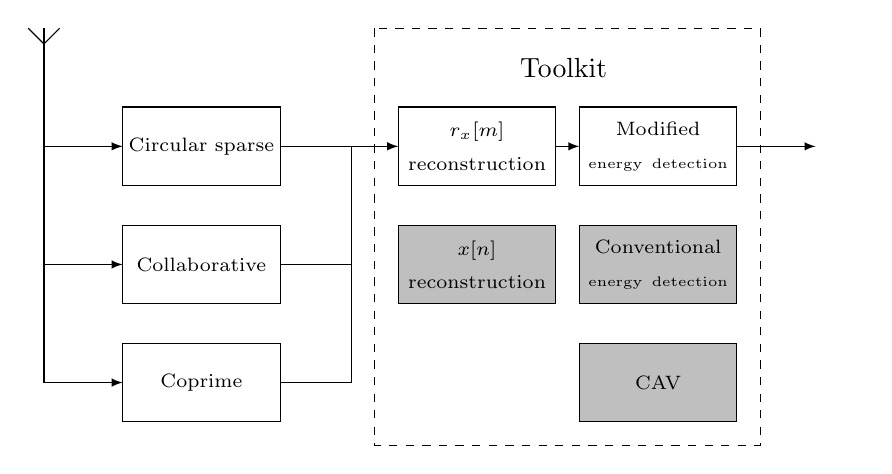
\begin{tikzpicture}
\draw  (-2,3) rectangle (0,2) node[pos=.5]{\scriptsize Circular sparse};
\draw  (-2,1.5) rectangle (0,0.5) node[pos=.5]{\scriptsize Collaborative};
\draw  (-2,0) rectangle (0,-1) node[pos=.5]{\scriptsize Coprime};
\draw  (1.5,3) rectangle (3.5,2) node[text width=5cm, align=center,pos=.5]{\scriptsize $r_x[m]$\\ reconstruction};
% \draw  [fill=lightgray] (1.5,0) rectangle (3.5,-1) node[text width=5cm, align=center,pos=.5]{\scriptsize $r_x$\\ reconstruction};
\draw  [fill=lightgray](1.5,1.5) rectangle (3.5,0.5) node[text width=5cm, align=center,pos=.5]{\scriptsize $x[n]$\\ reconstruction};
\draw  (3.8,3) rectangle (5.8,2) node[text width=5cm, align=center,pos=.5]{\scriptsize Modified\\\tiny energy detection};
\draw  [fill=lightgray] (3.8,1.5) rectangle (5.8,0.5) node[text width=5cm, align=center,pos=.5]{\scriptsize Conventional\\\tiny energy detection};
\draw  [fill=lightgray](3.8,0) rectangle (5.8,-1) node[pos=.5]{\scriptsize CAV};
\draw  [dashed] (1.2,4) rectangle (6.1,-1.3);
\node at (3.6,3.5) {Toolkit};
\draw [>=latex,->] (3.5,2.5) -- (3.8,2.5);
\draw [>=latex,->] (5.8,2.5) -- (6.8,2.5);
\draw [>=latex,->] (0,2.5) -- (1.5,2.5);
\draw [>=latex,->] (-3,2.5) -- (-2,2.5);
\draw [>=latex,->] (-3,1) -- (-2,1);
\draw [>=latex,->] (-3,-0.5) -- (-2,-0.5);
\draw (0,-0.5) -- (0.9,-0.5);
\draw (0,1) -- (0.9,1);
\draw (-3,-0.5) -- (-3,4);
\draw (0.9,-0.5) -- (0.9,2.5);
\draw (-2.8,4) -- (-3,3.8);
\draw (-3.2,4) -- (-3,3.8);
\node at (3.5,3) {};
\end{tikzpicture}
\caption{System overview with design choices}
\label{fig:theoretical_overview_system}
\end{figure}

\section{Testing}
To evaluate the performance of our system we will we use an artificial testing signal to test both the reconstructor and the detector.
Details on this signal generation can be found the subsequent section.

\subsection{Test signal}\label{ssec:test_signal}
The test signal will consist of an ideal signal contaminated with noise. The signal power and noise power will be based on a specified signal-to-noise ratio. Given a signal-to-noise ratio, we can construct the testing signal by doing as follows:

\begin{enumerate}
	\item Generate the ideal signal $s[n]$. The signal will consist of filtered circular symmetric complex Gaussian noise such that it represents a bandpass signal with $-0.2 \leq f\leq 0.2$, where $f$ denotes the usual relative frequency. The average power of the signal at frequencies in the passband is chosen such that the required SNR will be met. 
	\item Generate the noise signal $w[n]$, which will be additive circular symmetric complex Gaussian noise.
	\item Add $s[n]$ to $w[n]$ to produce the testing signal $x[n]$.
\end{enumerate}

\subsection{Tests}
There are three parameters of the system, represented by circles in \cref{tkz:test_system}, that will be used in our tests to assess the performance of the system. The parameters are as follows:
\begin{enumerate}
	\item The SNR of the input signal.
	\item The sampler type used to sample the input signal.
	\item The false alarm probability $p\ss{fa}$ of the detector.
\end{enumerate}

\begin{figure}
	\centerline{
	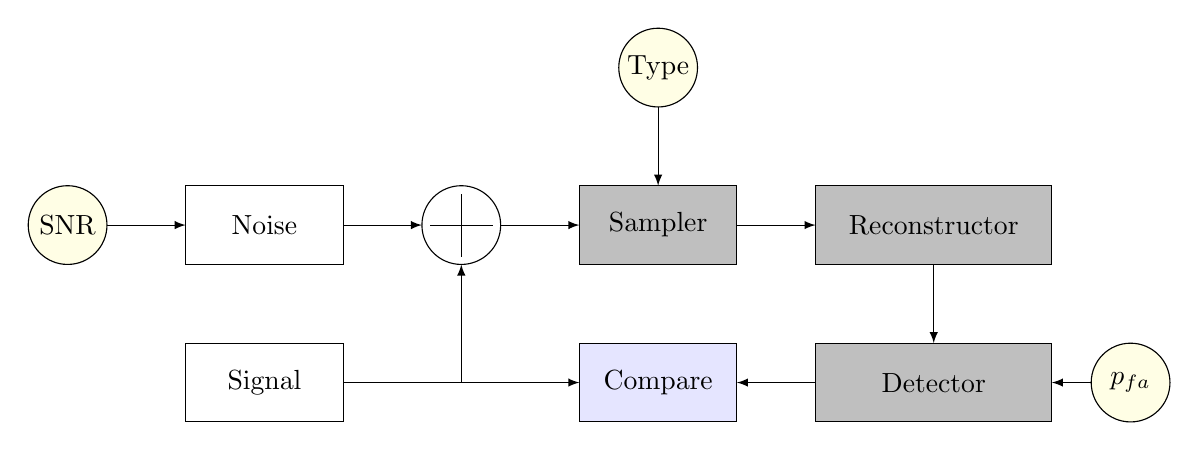
\begin{tikzpicture}
	\draw  (-2,3.5) rectangle (0,2.5) node[pos=.5]{Noise};
	\draw  (-2,1.5) rectangle (0,0.5) node[pos=.5]{Signal};
	\draw  (1.5,3) ellipse (.5 and .5);
	\draw  [fill=lightgray](3,3.5) rectangle (5,2.5) node[pos=.5]{Sampler};
	\draw  [fill=lightgray](6,3.5) rectangle (9,2.5) node[pos=.5]{Reconstructor};
	\draw  [fill=lightgray](6,1.5) rectangle (9,0.5) node[pos=.5]{Detector};
	\draw  [fill=blue, opacity=.1](3,1.5) rectangle (5,0.5);
	\draw  (3,1.5) rectangle (5,0.5)node[pos=.5]{Compare};
	\draw (1.5,2.6) -- (1.5,3.4);
	\draw (1.9,3) -- (1.1,3);
	\draw [>=latex, ->] (0,3) -- (1,3);
	\draw [>=latex, ->] (9.5,1) -- (9,1);
	\draw [>=latex, ->] (4,4.5) -- (4,3.5);
	\draw [>=latex, ->] (1.5,1) -- (1.5,2.5);
	\draw [>=latex, ->] (-3,3) -- (-2,3);
	\draw [>=latex, ->] (6,1) -- (5,1);
	\draw [>=latex, ->] (0,1) -- (3,1);
	\draw [>=latex, ->] (7.5,2.5) -- (7.5,1.5);
	\draw [>=latex, ->] (2,3) -- (3,3);
	\draw [>=latex, ->] (5,3) -- (6,3);
	\draw   [fill=yellow, opacity=.1] (-3.5,3) ellipse (.5 and .5);
	\draw   [fill=yellow, opacity=.1] (10,1) ellipse (.5 and .5);
	\draw   [fill=yellow, opacity=.1] (4,5) ellipse (.5 and .5);
	\draw   (-3.5,3) ellipse (.5 and .5) node{SNR};
	\draw  (10,1) ellipse (.5 and .5) node{$p_{fa}$};
	\draw  (4,5) ellipse (.5 and .5) node{Type};
	\end{tikzpicture}}
	\caption{Testing the system}\label{tkz:test_system}
\end{figure}

Our tests will be targeted at
\begin{enumerate}
	\item addressing the performance of the reconstruction by feeding it an artificial constructed signal while
	\begin{enumerate}
		\item varying the sampling technique used to sample the signal, described in \cref{cha:sampling_methods} and
		\item varying the compression rate and the sampling time, described in \cref{cha:reconstruction}.
	\end{enumerate}
	By comparing the reconstructed power spectral density to the power spectral density recovered directly from the constructed test signal, we can evaluate the correctness of reconstruction when used with a specific sampling technique.
	% Furthermore the dependence on the sampling time and the compression factor can be evaluated from those test results. 
	\item addressing the performance of detection on the reconstructed signal. The modified energy detector as described in \cref{ssec:ari_ed} will be evaluated by tests that make use of the test signal as described in \cref{ssec:test_signal}. 
	Detection is applied to the output of the reconstructor while	
	\begin{enumerate}
		\item varying the signal-to-noise ratio of the test signal and
		\item varying the false alarm probability the detector 
		should allow.
	\end{enumerate}

	The sampling technique is fixed to circular sparse sampling. The reason for this is that the dependence of the detector's performance on the reconstructor's performance, is such that techniques with equivalent reconstruction performance yield approximately equivalent detection performance. Therefore, we can use the results of the reconstructor to extrapolate the results of the detector.

	By extensive simulation we can construct estimates of the \emph{receiver operating characteristic curves}, which plot the detection probability versus the false alarm probability of the detector. From these curves the minimum signal strength and the detectors performance on a random signal can be evaluated. Furthermore the detection performance of the system as a whole can be evaluated by comparing these curves.
	\end{enumerate}

\section{Results}
The performance of the reconstructor is depicted in \cref{fig:plot-nmse-cop,fig:plot-nmse-circ,fig:plot-nmse}, which are accompanied by \cref{tab:sampling-nmse,tab:sampling-nmse-cop,tab:sampling-nmse-circ}. The performance of the detector is depicted in \cref{fig:plot-detector-noise76,fig:plot-detector76,fig:plot-detector-noise69,fig:plot-detector69}. Their results will be evaluated separately. Before we continue, the reader must be aware of the following two concepts.

First, we argued in the introduction the we want to avoid sampling at the Nyquist frequency. It turned out that multi-coset sampling offered a solution to this problem. To evaluate the different sampling techniques, we introduce a quantity called \textit{compression}. Compression is the percentage of samples the sampling technique requires with respect to the samples obtained when sampling at the Nyquist frequency. Therefore, high compression represents an effective sampling technique.

Second, we introduce the normalised mean squared error (NMSE) to assess the performance of the reconstructed power spectral density.\footnote{If $\hat{\text{PSD}}$ represents the estimated power spectral density, then the NMSE is given by $\text{NMSE} = ||\text{PSD} - \hat{\text{PSD}}||/||\text{PSD}||$.} A lower NMSE represents a better reconstruction of the power spectral density.

\subsection{Reconstruction}
The performance of the reconstruction will by measured by varying the sampling time, where we illustratively assume a Nyquist frequency of \SI{25}{Mhz}, and by varying the sampling technique. These sampling techniques can all achieve different compressions.

\cref{fig:plot-nmse-cop} shows the NSME for coprime sampling. We see that the error increases as the compression increases, but decreases as the sampling time increases. A similar observation applies to \cref{fig:plot-nmse-circ}. Also, we see that for a similar compression, circular sparse ruler provides less error than coprime sampling. The precise configuration is described in \cref{tab:sampling-nmse-cop,tab:sampling-nmse-circ}. These tables show us that circular sparse ruler allows for more downsampling, but also requires more samplers. Note that the resolutions of the reconstructed spectra differ. This should be taken into account when comparing the two methods. \cref{fig:plot-nmse} shows three sampling techniques which have equivalent performance. We observe that their performance gain by increasing the sampling time is equivalent. \cref{tab:sampling-nmse} shows that in the case of equivalent performance, coprime sampling requires the least number of samplers. Also, in that case, coprime sampling has the least downsampling and circular sparse ruler sampling has the highest compression.

\subsection{Detection}
\cref{fig:plot-detector-noise69,fig:plot-detector69} show the performance of the detector in the case that circular sparse ruler sampling with $69\%$ compression is used. The performance is shown for signals with \SI{-5}{dB}, \SI{0}{dB} and \SI{5}{dB} SNR. In addition to detection using the theoretical noise level, we have simulated uncertainty in noise power by adding \SI{0.5}{dB} to the theoretical noise level.

The 802.22 IEEE standard tells us that a detection probability of $0.9$ can be considered sufficient. We see that in case that the noise power is known, signals with approximately \SI{0}{dB} SNR or higher can be detected sufficiently. However, in the case that the noise power is not accurately known, a detection probability of approximately $0.9$ requires a relatively high false-alarm probability. Finally, if we increase the compression of the used sampling technique, the detection performance deteriorates.

%%%%%% PLOT: ALL SAMPLING METHODS
\begin{filecontents*}{plots/data-nyq.csv}
x,y
1.0000,-1.1522
2.0000,-1.3064
3.0000,-1.3805
4.0000,-1.4545
5.0000,-1.4858
6.0000,-1.5429
7.0000,-1.5787
8.0000,-1.6031
9.0000,-1.6351
10.0000,-1.6413
11.0000,-1.6651
12.0000,-1.6934
13.0000,-1.7020
14.0000,-1.7290
15.0000,-1.7354
16.0000,-1.7281
17.0000,-1.7755
18.0000,-1.7692
19.0000,-1.7853
20.0000,-1.7851
\end{filecontents*}

\begin{filecontents*}{plots/data-circ1.csv}
x, y
1.0000,-0.8209
2.0000,-0.9527
3.0000,-1.0311
4.0000,-1.0955
5.0000,-1.1467
6.0000,-1.1722
7.0000,-1.2186
8.0000,-1.2394
9.0000,-1.2612
10.0000,-1.2822
11.0000,-1.3134
12.0000,-1.3362
13.0000,-1.3494
14.0000,-1.3585
15.0000,-1.3660
16.0000,-1.3992
17.0000,-1.3952
18.0000,-1.4198
19.0000,-1.4276
20.0000,-1.4377
\end{filecontents*}


\begin{filecontents*}{plots/data-copr.csv}
x, y
1.0000,-0.8194
2.0000,-0.9547
3.0000,-1.0277
4.0000,-1.0808
5.0000,-1.1364
6.0000,-1.1707
7.0000,-1.1929
8.0000,-1.2289
9.0000,-1.2551
10.0000,-1.2720
11.0000,-1.2990
12.0000,-1.3191
13.0000,-1.3344
14.0000,-1.3566
15.0000,-1.3575
16.0000,-1.3770
17.0000,-1.3936
18.0000,-1.4071
19.0000,-1.4092
20.0000,-1.4196
\end{filecontents*}

\begin{filecontents*}{plots/data-collab.csv}
x, y
1.0000,-0.8216
2.0000,-0.9448
3.0000,-1.0348
4.0000,-1.1092
5.0000,-1.1430
6.0000,-1.1786
7.0000,-1.2148
8.0000,-1.2502
9.0000,-1.2717
10.0000,-1.3018
11.0000,-1.3077
12.0000,-1.3185
13.0000,-1.3578
14.0000,-1.3680
15.0000,-1.3903
16.0000,-1.3937
17.0000,-1.4090
18.0000,-1.4122
19.0000,-1.4355
20.0000,-1.4437
\end{filecontents*}


\begin{table}
	\centerline{
	\begin{tabular}{llll}
		\textbf{Sampling technique} & \textbf{Compression} & \textbf{Configuration} & \textbf{Downsampling} \\ \hline
		Circular sparse ruler sampling & $69\%$ & $4$ samplers & $13 \times$ \\
		Coprime sampling & $55\%$ & $2$ samplers, periods $4T$ and $5T$ & $4 \times$ \\
		Collaborative & $54\%$ &$6$ samplers over $2$ devices & $13 \times$
	\end{tabular}}
	\caption{Description of the sampling techniques depicted in \cref{fig:plot-nmse}}
	\label{tab:sampling-nmse}
\end{table}

%%%%%%


%%%%% PLOT: CIRCULAR
\begin{filecontents*}{plots/data-circ-N7.csv}
x, y
1.0000,-1.0770
2.0000,-1.2115
3.0000,-1.3001
4.0000,-1.3641
5.0000,-1.4234
6.0000,-1.4626
7.0000,-1.4847
8.0000,-1.5209
9.0000,-1.5396
10.0000,-1.5523
11.0000,-1.5902
12.0000,-1.5941
13.0000,-1.6163
14.0000,-1.6500
15.0000,-1.6521
16.0000,-1.6613
17.0000,-1.6849
18.0000,-1.6858
19.0000,-1.7015
20.0000,-1.6896
\end{filecontents*}

\begin{filecontents*}{plots/data-circ-N13.csv}
x, y
1.0000,-0.8209
2.0000,-0.9527
3.0000,-1.0311
4.0000,-1.0955
5.0000,-1.1467
6.0000,-1.1722
7.0000,-1.2186
8.0000,-1.2394
9.0000,-1.2612
10.0000,-1.2822
11.0000,-1.3134
12.0000,-1.3362
13.0000,-1.3494
14.0000,-1.3585
15.0000,-1.3660
16.0000,-1.3992
17.0000,-1.3952
18.0000,-1.4198
19.0000,-1.4276
20.0000,-1.4377
\end{filecontents*}

\begin{filecontents*}{plots/data-circ-N21.csv}
x, y
1.0000,-0.6166
2.0000,-0.7633
3.0000,-0.8441
4.0000,-0.9097
5.0000,-0.9474
6.0000,-0.9802
7.0000,-1.0162
8.0000,-1.0426
9.0000,-1.0565
10.0000,-1.0919
11.0000,-1.1013
12.0000,-1.1186
13.0000,-1.1354
14.0000,-1.1497
15.0000,-1.1679
16.0000,-1.1779
17.0000,-1.1974
18.0000,-1.2134
19.0000,-1.2264
20.0000,-1.2294
\end{filecontents*}


\begin{table}
	\centerline{
	\begin{tabular}{llll}
		\textbf{Sampling technique} & \textbf{Compression} & \textbf{Configuration} & \textbf{Downsampling} \\ \hline
		Circular sparse ruler sampling & $57\%$ & $3$ samplers & $7 \times$ \\
		Circular sparse ruler sampling & $69\%$ & $4$ samplers & $13 \times$ \\
		Circular sparse ruler sampling & $76\%$ & $5$ samplers & $21 \times$ \\
	\end{tabular}}
	\caption{Description of the sampling techniques depicted in \cref{fig:plot-nmse-circ}}
	\label{tab:sampling-nmse-circ}
\end{table}

%%%%%%%

%%%%%% PLOT: COPRIME

\begin{filecontents*}{plots/data-cop-35.csv}
x, y
1.0000,-0.9237
2.0000,-1.0522
3.0000,-1.1518
4.0000,-1.2059
5.0000,-1.2442
6.0000,-1.2868
7.0000,-1.3234
8.0000,-1.3534
9.0000,-1.3860
10.0000,-1.4091
11.0000,-1.4210
12.0000,-1.4332
13.0000,-1.4595
14.0000,-1.4768
15.0000,-1.4898
16.0000,-1.4959
17.0000,-1.5101
18.0000,-1.5366
19.0000,-1.5400
20.0000,-1.5497
\end{filecontents*}

\begin{filecontents*}{plots/data-cop-45.csv}
x, y
1.0000,-0.8194
2.0000,-0.9547
3.0000,-1.0277
4.0000,-1.0808
5.0000,-1.1364
6.0000,-1.1707
7.0000,-1.1929
8.0000,-1.2289
9.0000,-1.2551
10.0000,-1.2720
11.0000,-1.2990
12.0000,-1.3191
13.0000,-1.3344
14.0000,-1.3566
15.0000,-1.3575
16.0000,-1.3770
17.0000,-1.3936
18.0000,-1.4071
19.0000,-1.4092
20.0000,-1.4196
\end{filecontents*}

\begin{filecontents*}{plots/data-cop-47.csv}
x, y
1.0000,-0.6748
2.0000,-0.8165
3.0000,-0.9064
4.0000,-0.9664
5.0000,-1.0057
6.0000,-1.0463
7.0000,-1.0715
8.0000,-1.0929
9.0000,-1.1218
10.0000,-1.1523
11.0000,-1.1631
12.0000,-1.1766
13.0000,-1.2022
14.0000,-1.2157
15.0000,-1.2229
16.0000,-1.2400
17.0000,-1.2527
18.0000,-1.2664
19.0000,-1.2811
20.0000,-1.2861
\end{filecontents*}

\begin{table}
	\centerline{
	\begin{tabular}{llll}
		\textbf{Sampling technique} & \textbf{Compression} & \textbf{Configuration} & \textbf{Downsampling} \\ \hline
		Corpime sampling & $47\%$ & $2$ samplers, periods $3T$ and $5T$ & $3 \times$ \\
		Corpime sampling & $55\%$ & $2$ samplers, periods $4T$ and $5T$ & $4 \times$ \\
		Corpime sampling & $612\%$ & $2$ samplers, periods $4T$ and $7T$ & $4 \times$ \\
	\end{tabular}}
	\caption{Description of the sampling techniques depicted in \cref{fig:plot-nmse-cop}}
	\label{tab:sampling-nmse-cop}
\end{table}


%%%%%%%%



%%%%%% PLOT: RECONSTRUCTOR ALL

\begin{figure}
	\centerline{
	\begin{subfigure}[t]{0.4\paperwidth}
		\centering
		\begin{tikzpicture}
			\begin{axis}[
					xlabel={Sampling time (ms)},
					ylabel={$\log_{10}(\text{NMSE})$},
					width=8cm,
					height=8cm,
					scale=1,
					grid=both,
					axis lines=left,
					legend entries={$0\%$ compression,$47\%$ compression, $55\%$ compression, $61\%$ compression},
					legend cell align=left
				]
			    \addplot [
				    color=black,
				    solid,
				    mark=o
			    ] table [x=x, y=y, col sep=comma]{plots/data-nyq.csv};
			    \addplot [
				    color=red,
				    solid,
				    mark=o
			    ] table [x=x, y=y, col sep=comma]{plots/data-cop-35.csv};
			    \addplot [
				    color=green,
				    solid,
				    mark=o
			    ] table [x=x, y=y, col sep=comma]{plots/data-cop-45.csv};
			    \addplot [
				    color=blue,
				    solid,
				    mark=o
			    ] table [x=x, y=y, col sep=comma]{plots/data-cop-47.csv};
			\end{axis}
		\end{tikzpicture}
		\caption{Coprime sampling. The curves are described in \cref{tab:sampling-nmse-cop}.}
		\label{fig:plot-nmse-cop}
	\end{subfigure}
	\begin{subfigure}[t]{0.4\paperwidth}
		\centering
		\begin{tikzpicture}
			\begin{axis}[
					xlabel={Sampling time (ms)},
					ylabel={$\log_{10}(\text{NMSE})$},
					width=8cm,
					height=8cm,
					scale=1,
					grid=both,
					axis lines=left,
					legend entries={$0\%$ compression,$57\%$ compression, $69\%$ compression, $76\%$ compression},
					legend cell align=left
				]
			    \addplot [
				    color=black,
				    solid,
				    mark=o
			    ] table [x=x, y=y, col sep=comma]{plots/data-nyq.csv};
			    \addplot [
				    color=red,
				    solid,
				    mark=o
			    ] table [x=x, y=y, col sep=comma]{plots/data-circ-N7.csv};
			    \addplot [
				    color=green,
				    solid,
				    mark=o
			    ] table [x=x, y=y, col sep=comma]{plots/data-circ-N13.csv};
			    \addplot [
				    color=blue,
				    solid,
				    mark=o
			    ] table [x=x, y=y, col sep=comma]{plots/data-circ-N21.csv};
			\end{axis}
		\end{tikzpicture}
		\caption{Circular sparse sampling. The curves are described in \cref{tab:sampling-nmse-circ}.}
		\label{fig:plot-nmse-circ}
	\end{subfigure}
	}
	\vspace{1cm}
	\centerline{
	\begin{subfigure}[t]{0.8\paperwidth}
		\centering
		\begin{tikzpicture}
			\begin{axis}[
					xlabel={Sampling time (ms)},
					ylabel={$\log_{10}(\text{NMSE})$},
					width=11cm,
					height=8cm,
					scale=1,
					grid=both,
					axis lines=left,
					legend entries={Circular sparse sampling, Coprime sampling, Collorative sampling},
					legend cell align=left
				]
			    \addplot [
				    color=red,
				    solid,
				    mark=o
			    ] table [x=x, y=y, col sep=comma]{plots/data-circ1.csv};
			    % \addplot [
				   %  color=green,
				   %  solid,
				   %  mark=o
			    % ] table [x=x, y=y, col sep=comma]{plots/data-circ2.csv};
			    \addplot [
				    color=green,
				    solid,
				    mark=o
			    ] table [x=x, y=y, col sep=comma]{plots/data-copr.csv};
			    \addplot [
				    color=blue,
				    solid,
				    mark=o
			    ] table [x=x, y=y, col sep=comma]{plots/data-collab.csv};
			\end{axis}
		\end{tikzpicture}
		\caption{Equivalent performance of different techniques. The curves are described in \cref{tab:sampling-nmse}.}
		\label{fig:plot-nmse}
	\end{subfigure}
	}
	\caption{Normalised mean squared errors of the reconstructed power spectral densities by different sampling methods. The plots assume a Nyquist frequency of \SI{25}{MHz}. The Nyquist sampled signal is limited in support such that $r_x[m]=0$ for $|m| > 60$. Note that the different techniques yield different resolutions.}
\end{figure}




%%%%%






%%%%%% PLOT: DETECTOR

\begin{filecontents*}{plots/data-detector-snr-5-1.csv}
x, y
0.021752,0.238
0.041678,0.32307
0.062985,0.38559
0.082069,0.43566
0.1015,0.47798
\end{filecontents*}
\begin{filecontents*}{plots/data-detector-snr-5-2.csv}
x, y
0.00025373,0.022236
0.00089851,0.04471
0.0019284,0.068319
0.0033224,0.090696
0.0051313,0.11501
\end{filecontents*}
\begin{filecontents*}{plots/data-detector-snr0-1.csv}
x, y
0.022215,0.89002
0.042224,0.92428
0.062003,0.94177
0.081218,0.95271
0.1008,0.96058
\end{filecontents*}
\begin{filecontents*}{plots/data-detector-snr0-2.csv}
x, y
0.00027463,0.57327
0.00083582,0.66899
0.0019313,0.72643
0.0032418,0.76901
0.0051134,0.79744
\end{filecontents*}
\begin{filecontents*}{plots/data-detector-snr5-1.csv}
x, y
0.021576,0.99994
0.041976,0.99996
0.061913,0.99995
0.081218,0.99999
0.10079,0.99997
\end{filecontents*}
\begin{filecontents*}{plots/data-detector-snr5-2.csv}
x, y
0.00027463,0.99944
0.00095224,0.99964
0.0019254,0.99974
0.0032,0.99979
0.0050269,0.99984
\end{filecontents*}


\begin{figure}
	\centerline{
	\begin{subfigure}[t]{.4\paperwidth}
		\centering
		\begin{tikzpicture}
			\begin{axis}[
					scaled ticks=false, tick label style={/pgf/number format/fixed},
					xlabel={$p\ss{fa}$},
					ylabel={$p\ss{d}$},
					width=8cm,
					height=8cm,
					scale=1,
					grid=both,
					axis lines=left,
					legend entries={\SI{-5}{dB} SnR,\SI{0}{dB} SnR,\SI{5}{dB} SnR},
					legend cell align=left,
					% xmin=0.01,
					% xmax=0.105,
					ymin=0,
					ymax=1.05,
					legend style={at={(6.2cm,0.02)},anchor=south east}
				]
			    \addplot [
				    color=red,
				    solid,
				    mark=o
			    ] table [x=x, y=y, col sep=comma]{plots/data-detector-snr-5-1.csv};
			    \addplot [
				    color=green,
				    solid,
				    mark=o
			    ] table [x=x, y=y, col sep=comma]{plots/data-detector-snr0-1.csv};
			    \addplot [
				    color=blue,
				    solid,
				    mark=o
			    ] table [x=x, y=y, col sep=comma]{plots/data-detector-snr5-1.csv};
			\end{axis}
		\end{tikzpicture}
		\caption{The case of no noise power uncertainty}
		\label{fig:plot-detector76}
	\end{subfigure}
	\begin{subfigure}[t]{.4\paperwidth}
		\centering
		\begin{tikzpicture}
			\begin{axis}[
					xlabel={$p\ss{fa}$},
					ylabel={$p\ss{d}$},
					width=8cm,
					height=8cm,
					scale=1,
					grid=both,
					axis lines=left,
					legend entries={\SI{-5}{dB} SnR,\SI{0}{dB} SnR,\SI{5}{dB} SnR},
					legend cell align=left,
					% xmin=0,
					% xmax=0.12,
					y tick label style={/pgf/number format/fixed},
					ymin=0,
					ymax=1.05,
					legend style={at={(6.2cm,1cm)},anchor=south east}
				]
			    \addplot [
				    color=red,
				    solid,
				    mark=o
			    ] table [x=x, y=y, col sep=comma]{plots/data-detector-snr-5-2.csv};
			    \addplot [
				    color=green,
				    solid,
				    mark=o
			    ] table [x=x, y=y, col sep=comma]{plots/data-detector-snr0-2.csv};
			    \addplot [
				    color=blue,
				    solid,
				    mark=o
			    ] table [x=x, y=y, col sep=comma]{plots/data-detector-snr5-2.csv};
			\end{axis}
		\end{tikzpicture}
		\caption{The case of \SI{0.1}{dB} noise power uncertainty}
		\label{fig:plot-detector-noise76}
	\end{subfigure}
	}
	\caption{The detector's receiver operation characteristic. Circular sparse sampling with $76\%$ compression is used.}
\end{figure}

%%%%%%


%%%%%% PLOT: DETECTOR2

\begin{filecontents*}{plots/data-detector2-snr-5-1.csv}
x, y
0.021474,0.32638
0.041823,0.42309
0.062284,0.48659
0.081647,0.54171
0.101,0.58043
\end{filecontents*}
\begin{filecontents*}{plots/data-detector2-snr-5-2.csv}
x, y
8.8372e-05,0.024414
0.00034419,0.048884
0.00075349,0.072135
0.0014698,0.097842
0.0022512,0.11979
\end{filecontents*}
\begin{filecontents*}{plots/data-detector2-snr0-1.csv}
x, y
0.021549,0.94161
0.04126,0.956
0.061907,0.9622
0.081605,0.96686
0.1012,0.96985
\end{filecontents*}
\begin{filecontents*}{plots/data-detector2-snr0-2.csv}
x, y
0.00012093,0.73009
0.00031628,0.79912
0.00075349,0.83472
0.0014512,0.85859
0.0021628,0.87747
\end{filecontents*}
\begin{filecontents*}{plots/data-detector2-snr5-1.csv}
x, y
0.021507,0.99138
0.042312,0.99293
0.062512,0.99434
0.081367,0.99482
0.099693,0.99513
\end{filecontents*}
\begin{filecontents*}{plots/data-detector2-snr5-2.csv}
x, y
0.00012093,0.97744
0.00032093,0.98055
0.00086047,0.98304
0.0014047,0.98449
0.0022419,0.98557
\end{filecontents*}


\begin{figure}
	\centerline{
	\begin{subfigure}[t]{.4\paperwidth}
		\centering
		\begin{tikzpicture}
			\begin{axis}[
					scaled ticks=false, tick label style={/pgf/number format/fixed},
					xlabel={$p\ss{fa}$},
					ylabel={$p\ss{d}$},
					width=8cm,
					height=8cm,
					scale=1,
					grid=both,
					axis lines=left,
					legend entries={\SI{-5}{dB} SnR,\SI{0}{dB} SnR,\SI{5}{dB} SnR},
					legend cell align=left,
					% xmin=0.01,
					% xmax=0.105,
					ymin=0,
					ymax=1.05,
					legend style={at={(6.2cm,0.02)},anchor=south east}
				]
			    \addplot [
				    color=red,
				    solid,
				    mark=o
			    ] table [x=x, y=y, col sep=comma]{plots/data-detector2-snr-5-1.csv};
			    \addplot [
				    color=green,
				    solid,
				    mark=o
			    ] table [x=x, y=y, col sep=comma]{plots/data-detector2-snr0-1.csv};
			    \addplot [
				    color=blue,
				    solid,
				    mark=o
			    ] table [x=x, y=y, col sep=comma]{plots/data-detector2-snr5-1.csv};
			\end{axis}
		\end{tikzpicture}
		\caption{The case of no noise power uncertainty}
		\label{fig:plot-detector69}
	\end{subfigure}
	\begin{subfigure}[t]{.4\paperwidth}
		\centering
		\begin{tikzpicture}
			\begin{axis}[
					xlabel={$p\ss{fa}$},
					ylabel={$p\ss{d}$},
					width=8cm,
					height=8cm,
					scale=1,
					grid=both,
					axis lines=left,
					legend entries={\SI{-5}{dB} SnR,\SI{0}{dB} SnR,\SI{5}{dB} SnR},
					legend cell align=left,
					% xmin=0,
					% xmax=0.12,
					y tick label style={/pgf/number format/fixed},
					ymin=0,
					ymax=1.05,
					legend style={at={(6.2cm,1cm)},anchor=south east}
				]
			    \addplot [
				    color=red,
				    solid,
				    mark=o
			    ] table [x=x, y=y, col sep=comma]{plots/data-detector2-snr-5-2.csv};
			    \addplot [
				    color=green,
				    solid,
				    mark=o
			    ] table [x=x, y=y, col sep=comma]{plots/data-detector2-snr0-2.csv};
			    \addplot [
				    color=blue,
				    solid,
				    mark=o
			    ] table [x=x, y=y, col sep=comma]{plots/data-detector2-snr5-2.csv};
			\end{axis}
		\end{tikzpicture}
		\caption{The case of \SI{0.1}{dB} noise power uncertainty}
		\label{fig:plot-detector-noise69}
	\end{subfigure}
	}
	\caption{The detector's receiver operation characteristic. Circular sparse sampling with $69\%$ compression is used.}
\end{figure}

%%%%%%





\end{document}
